% ============================================================
%  CHAPTER 1 : INTRODUCTION
% ============================================================
\chapter{Introduction}
\label{ch:intro}

\section{Motivation}

For most of modern history, whenever two people who did not know each other wanted to exchange something of value---money, property records, medical data---they needed a trusted middleman to make it work. Banks verify that you have enough money before letting you send a payment. Government registries confirm who owns a piece of land. Hospitals keep your medical records behind locked systems.  These centralised systems work well \emph{most of the time}, but they have a fundamental weakness: they concentrate enormous power and responsibility in a single place. If that single place is compromised---by a technical failure, a corrupt employee, or a sophisticated attacker---the consequences can be devastating.

Consider the Punjab National Bank (PNB) fraud of 2018, one of the largest banking scams in Indian history. A small group of employees, in collusion with jeweller Nirav Modi, issued fraudulent \glspl{lou} worth over \rupmark 13,000 crore (approximately USD~1.8~billion). These letters were never recorded in the bank's \gls{cbs}, meaning the fraud went undetected for years~\cite{web:apptunix}. The scam was possible precisely \emph{because} the system was centralised: a handful of insiders could bypass the controls that everyone else trusted implicitly.

Blockchain technology offers a radically different approach. Instead of placing trust in a single institution, it distributes trust across an entire network of participants. Every transaction is recorded on a shared ledger that anyone can verify, no single party can alter, and no central point of failure can bring down. In the words of the technology's most famous proponent, Satoshi Nakamoto, the goal is ``a system for electronic transactions without relying on trust''~\cite{nakamoto2008bitcoin}.

\section{Centralised vs.\ Decentralised Systems}
\label{sec:cent-decent}

To appreciate what blockchain does differently, it helps to first understand the two paradigms it bridges. \Cref{fig:cent-vs-decent} illustrates the structural difference.

\begin{figure}[htbp]
\centering
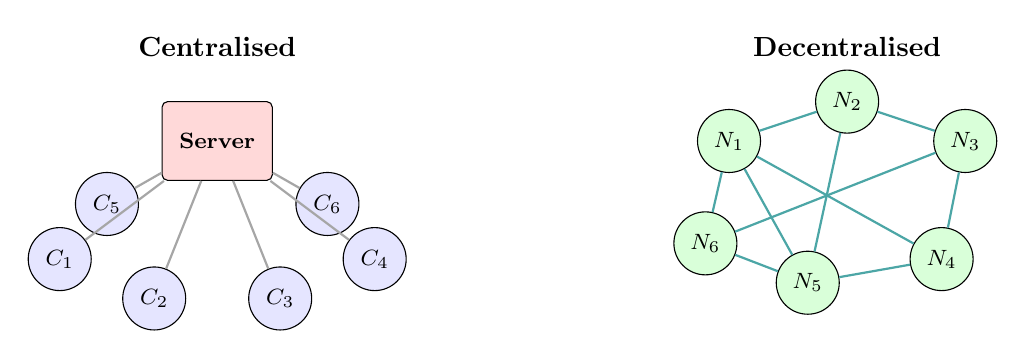
\begin{tikzpicture}[
    node distance=1.2cm,
    server/.style={rectangle, draw, fill=red!15, minimum width=1.4cm, minimum height=1cm, font=\footnotesize\bfseries, rounded corners=2pt},
    client/.style={circle, draw, fill=blue!10, minimum size=0.8cm, font=\footnotesize},
    peer/.style={circle, draw, fill=green!15, minimum size=0.8cm, font=\footnotesize},
    conn/.style={-, thick, gray!70},
    p2pconn/.style={-, thick, teal!70}
]

% --- Centralised ---
\node[font=\bfseries] at (-4, 3.2) {Centralised};
\node[server] (S) at (-4, 2) {Server};
\node[client] (C1) at (-6, 0.5) {$C_1$};
\node[client] (C2) at (-4.8, 0) {$C_2$};
\node[client] (C3) at (-3.2, 0) {$C_3$};
\node[client] (C4) at (-2, 0.5) {$C_4$};
\node[client] (C5) at (-5.4, 1.2) {$C_5$};
\node[client] (C6) at (-2.6, 1.2) {$C_6$};

\foreach \c in {C1,C2,C3,C4,C5,C6}
    \draw[conn] (S) -- (\c);

% --- Decentralised ---
\node[font=\bfseries] at (4, 3.2) {Decentralised};
\node[peer] (P1) at (2.5, 2) {$N_1$};
\node[peer] (P2) at (4, 2.5) {$N_2$};
\node[peer] (P3) at (5.5, 2) {$N_3$};
\node[peer] (P4) at (5.2, 0.5) {$N_4$};
\node[peer] (P5) at (3.5, 0.2) {$N_5$};
\node[peer] (P6) at (2.2, 0.7) {$N_6$};

\draw[p2pconn] (P1) -- (P2);
\draw[p2pconn] (P2) -- (P3);
\draw[p2pconn] (P3) -- (P4);
\draw[p2pconn] (P4) -- (P5);
\draw[p2pconn] (P5) -- (P6);
\draw[p2pconn] (P6) -- (P1);
\draw[p2pconn] (P1) -- (P5);
\draw[p2pconn] (P2) -- (P5);
\draw[p2pconn] (P3) -- (P6);
\draw[p2pconn] (P1) -- (P4);

\end{tikzpicture}
\caption{Centralised vs.\ decentralised network topologies. In a centralised system (left), all clients depend on a single server---a single point of failure. In a decentralised system (right), every node connects to multiple peers, so the network remains functional even if several nodes go offline.}
\label{fig:cent-vs-decent}
\end{figure}

\textbf{Centralised systems} are architectures in which a single authority controls data storage, transaction validation, and access permissions.  Examples include traditional banks, social media platforms such as Facebook (Meta), and cloud services like Google.  While efficient, they suffer from a critical vulnerability: a single point of failure.  If the central server is compromised, the entire system is affected.

\textbf{Decentralised systems} distribute control across many independent nodes. There is no single entity that can unilaterally alter, censor, or shut down the network.  Data is replicated across nodes, making the system highly resilient to failures and attacks.  Blockchain is the most prominent technology enabling such decentralisation for transactional data.

\Cref{tab:cent-vs-decent} summarises the key differences.

\begin{table}[htbp]
\centering
\renewcommand{\arraystretch}{1.3}
\begin{tabularx}{\textwidth}{l X X}
\toprule
\textbf{Property} & \textbf{Centralised} & \textbf{Decentralised} \\
\midrule
Control          & Single authority             & Distributed among all participants \\
Point of failure & Single (the central server)  & None (network tolerates node failures) \\
Transparency     & Opaque to end users          & Fully auditable by anyone \\
Trust model      & Trust in the institution     & Trust in the protocol and mathematics \\
Examples         & Banks, Google, Facebook      & Bitcoin, Ethereum \\
\bottomrule
\end{tabularx}
\caption{Comparison of centralised and decentralised systems.}
\label{tab:cent-vs-decent}
\end{table}

\section{What Is a Blockchain?}
\label{sec:what-is}

At its simplest, a \textbf{blockchain} is a continuously growing list of records---called \emph{blocks}---that are linked together using cryptographic hashes. Each block contains a batch of transactions, a timestamp, and the hash of the previous block, forming an unbroken chain stretching all the way back to the very first block (the \emph{genesis block}).

The key properties that make this simple structure so powerful are:

\begin{enumerate}
    \item \textbf{Immutability.} Once data is recorded in a block and the block is added to the chain, it cannot be changed or deleted without redoing all subsequent work---a computationally prohibitive task.
    \item \textbf{Decentralisation.} No single authority controls the blockchain. Instead, a network of nodes collectively maintains the ledger.
    \item \textbf{Transparency.} The ledger is public; anyone can verify any transaction at any time.
    \item \textbf{Resilience.} Because the same data exists on thousands of nodes worldwide, the system has no single point of failure.
\end{enumerate}

Put differently: in a blockchain system, \emph{trust is enforced by the system itself}---through transparency and mathematics---rather than by people or institutions.

\section{Our Contributions}

This report provides a self-contained, accessible introduction to blockchain technology. Our specific contributions are:

\begin{itemize}
    \item A clear explanation of the historical foundations of blockchain, from hash chains (1991) through Bit Gold (1998) to the Bitcoin whitepaper (2008)---see \Cref{ch:background}.
    \item A detailed walkthrough of how Bitcoin transactions, timestamp servers, and Proof of Work operate, written for readers without a prior background in cryptography---see \Cref{ch:background}.
    \item A comparative analysis of consensus mechanisms (PoW, PoS, PBFT) and scalability solutions (sharding, Layer~2, rollups)---see \Cref{ch:consensus}.
    \item A survey of real-world blockchain applications and advanced directions including smart contracts, zero-knowledge proofs, and cross-chain communication---see \Cref{ch:applications}.
    \item A discussion of the open challenges facing blockchain adoption and a formal treatment of the Blockchain Trilemma---see \Cref{ch:challenges}.
\end{itemize}

\section{Report Organisation}

The remainder of this report is organised as follows:
\begin{description}
    \item[\Cref{ch:background}] presents the historical and technical foundations: pre-2008 work, the Bitcoin protocol, and core cryptographic primitives.
    \item[\Cref{ch:consensus}] examines consensus mechanisms and scalability engineering.
    \item[\Cref{ch:applications}] surveys advanced directions and real-world applications.
    \item[\Cref{ch:challenges}] discusses open challenges and the Blockchain Trilemma.
    \item[\Cref{ch:conclusion}] concludes the report and outlines future research directions.
\end{description}
